\documentclass[11pt]{article}
\usepackage[portuguese]{babel}
\usepackage[T1]{fontenc}
\usepackage[a4paper, margin=2cm]{geometry}
\usepackage{authblk}
\usepackage{color}
\usepackage{listings}
\usepackage{setspace}
\usepackage{fontspec}
\usepackage{soul}
\usepackage{graphicx}
\usepackage{subcaption}
\usepackage{verbatimbox}

\setcounter{secnumdepth}{0}
\onehalfspacing
\setmainfont{Nimbus Sans}

\title{TRABALHO 1 - SEMESTRE 2022.2}
\author[1]{Pedro Santi Binotto [20200634]\thanks{\texttt{pedro.binotto@grad.ufsc.br}}}
\author[1]{Tales Antunes Mendes [20200636]\thanks{\texttt{talesmendes@hotmail.br}}}
\author[1]{Mateus Silva Teixeira [20200634]\thanks{\texttt{mateus.silva.teixeira@grad.ufsc.br}}}
\date{\today}

\affil[1]{Departamento de Informática e Estatística, Universidade Federal de Santa Catarina}

\begin{document}
\maketitle

\begin{abstract}
Este artigo tem o fim de estudar a relação entre o volume de iterações de
processamento realizados por uma aplicação e o tempo de computação necessário
para a conclusão da mesma, e à partir da análise dos dados resultantes,
comparar a performance da mesma tarefa implementada em diferentes linguagens de
programação, assim como projetar o tempo de processamento dos programas com um
número de iterações maior do que o volume utilizado nos testes de referência
através de modelos de regressão linear simples.
\end{abstract}

\newpage
\section{Introdução e Objetivos}
\paragraph{}
Historicamente, um dos maiores, se não o maior objetivo da pesquisa científica
na área da computação tem sido a otimização de performance de processamento,
tanto em termos de hardware\cite{schaller1997moore}, quanto na implementação de
software e linguagens de programação.

\paragraph{}
Em anos recentes, no entanto, avanços tecnológicos na construção de circuitos
de silício têm potencializado a utilização de linguagens de alto nível
\cite{srinath2017python}, que promovem a acessibilidade destas ferramentas
àqueles não familiarizados aos detalhes técnicos do desenvolvimento de software,
mas requisitam uma maior quantidade de recursos computacionais.

\paragraph{}
Todavia, a adoção destas facilidades representa, muitas vezes, um impacto
negativo na performance de computação de aplicações implementadas utilizando
estas linguagens\cite{prechelt2000empirical}. Naturalmente, surge a questão de
\textit{quando} pode ser considerado apropriado utilizar estas ferramentas para
realizar dada tarefa.

\paragraph{}
Portanto, este estudo foi realizado na tentativa de quantificar, visualizar, e
projetar a forma em que diferentes linguagens (compiladas, interpretadas, e
linguagens tipo \textit{bytecode}/virtualizadas) comportam-se sob crescentes
cargas de complexidade computacional.

\newpage
\section{Materiais e Métodos}
\paragraph{}
Para a realização deste estudo, foram utilizadas três linguagens de programação
diferentes, todas as quais apresentam ampla adoção na indústria de tecnologia
atual\cite{cass20152015}, mas que apresentam características distintas em termos de paradigma de
programação, tipagem de variáveis (forte ou fraca), estilo de execução
(compilada, interpretada, e virtualizada/JIT), e gerenciamento de memória
(coleção de lixo ou gerenciamento manual). Neste caso, os experimentos foram
realizados com \textit{benchmarks} implementados em \textbf{C}, \textbf{Java}, e
\textbf{Lua}.

\begin{itemize}
    \item \textbf{C}: Linguagem estaticamente tipada 
        (tipagem forte); compilada; gerenciamento manual de memória.
    \item \textbf{Java}: Linguagem estaticamente tipada (tipagem forte);
        execução virtualizada (bytecode/JIT); coleção de lixo automática.
    \item \textbf{Lua}: Linguagem dinamicamente tipada (tipagem fraca);
        execução interpretada; coleção de lixo automática.
\end{itemize}

\subsection{Especificações Técnicas}

\begin{verbatim}
C - Versão do compilador e configurações de ambiente.

clang version 13.0.1
Thread model: posix

Sem uso de flags de otimização adicionais.
\end{verbatim}

\hrule

\begin{verbatim}
Java - Versão do kit de desenvolvimento e runtime

openjdk version "1.8.0_302"
OpenJDK Runtime Environment (Zulu 8.56.0.21-CA-linux64) (build 1.8.0_302-b08)
OpenJDK 64-Bit Server VM (Zulu 8.56.0.21-CA-linux64) (build 25.302-b08, mixed mode)

Sem uso de flags de otimização adicionais.
\end{verbatim}

\hrule

\begin{verbatim}
Lua - Versão do interpretador

Lua 5.4.4  Copyright (C) 1994-2022 Lua.org, PUC-Rio

Sem uso de flags de otimização adicionais.
\end{verbatim}

\hrule

\begin{verbatim}
Ambiente e Hardware

OS: Manjaro Linux x86_64 
Kernel: 5.13.19-2-MANJARO 
CPU: AMD Ryzen 5 3500U with Radeon Vega Mobile Gfx (8) @ 2.100GHz 
RAM: 9892MiB 
\end{verbatim}

\newpage
\subsection{Testes de Performance}
\paragraph{}
Para coletar as métricas de tempo de processamento de cada linguagem, foram
implementados testes de complexidade temporal através de algoritmos de
multiplicação entre matrizes numéricas.
Os testes consistem na alocação de matrizes de mesma dimensão na memória do
sistema, e multiplicação de cada elemento através de iterações subsequentes,
produzindo um fator de complexidade temporal de
O(n\textsuperscript{3})\cite{stothers2010complexity}.

\paragraph{}
Para cada linguagem, foram realizados testes com cinco estágios diferentes de
carga computacional, de forma crescente, utilizando matrizes quadradas de
dimensões de 100, 500, 1000, 1500, e 2000 linhas, cada teste sendo repetido
cinco vezes, e temporizados com a utilidade padrão \texttt{time} de um sistema
UNIX (GNU time v2019-03-06).

\paragraph{}
É importante observar que, conforme ampliam-se as dimensões das matrizes
utilizadas, o número de elementos contidos na matriz cresce de forma
\textit{exponencial} em relação à contagem de linhas/colunas; e.g., ao
incrementar uma matriz de dimensões 100x100 para 200x200, a matriz em questão,
originalmente contendo 10.000 itens, passa a conter 40.000 elementos.

\newpage
\section{Resultados e Discussão}

\begin{figure}[!ht]
    \centering
    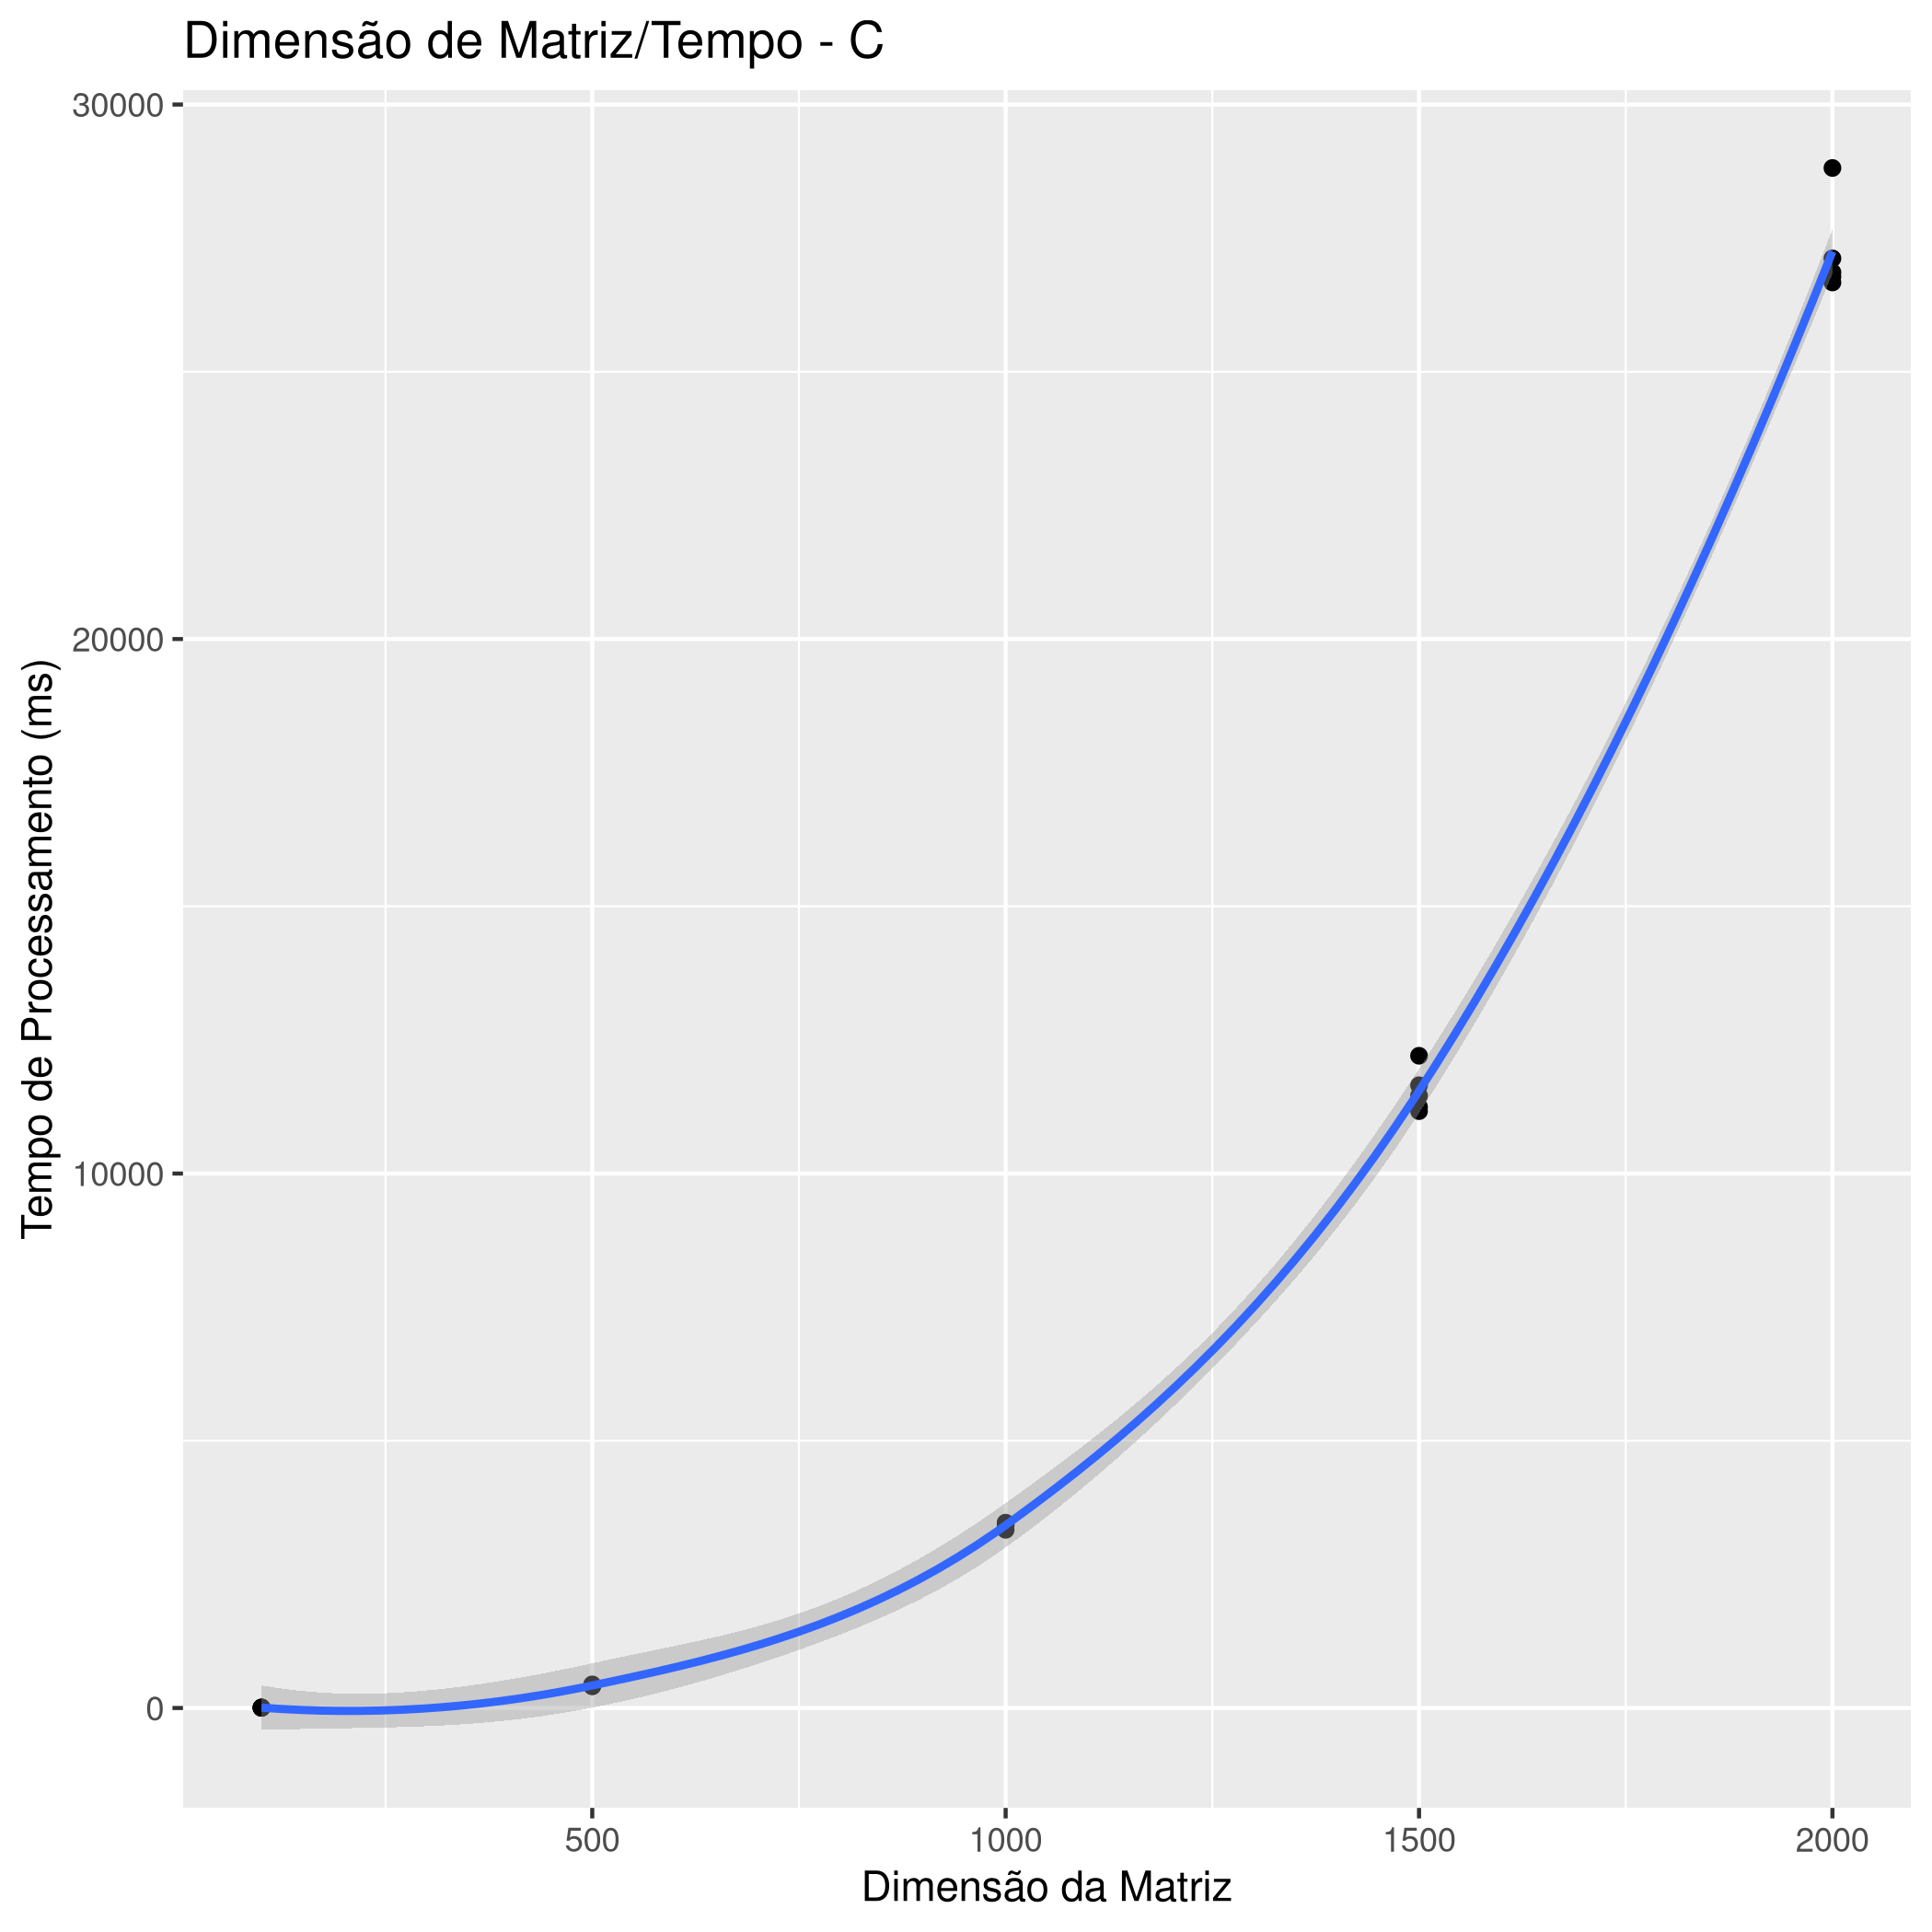
\includegraphics[width =0.3\textwidth]{plot_c.png}
    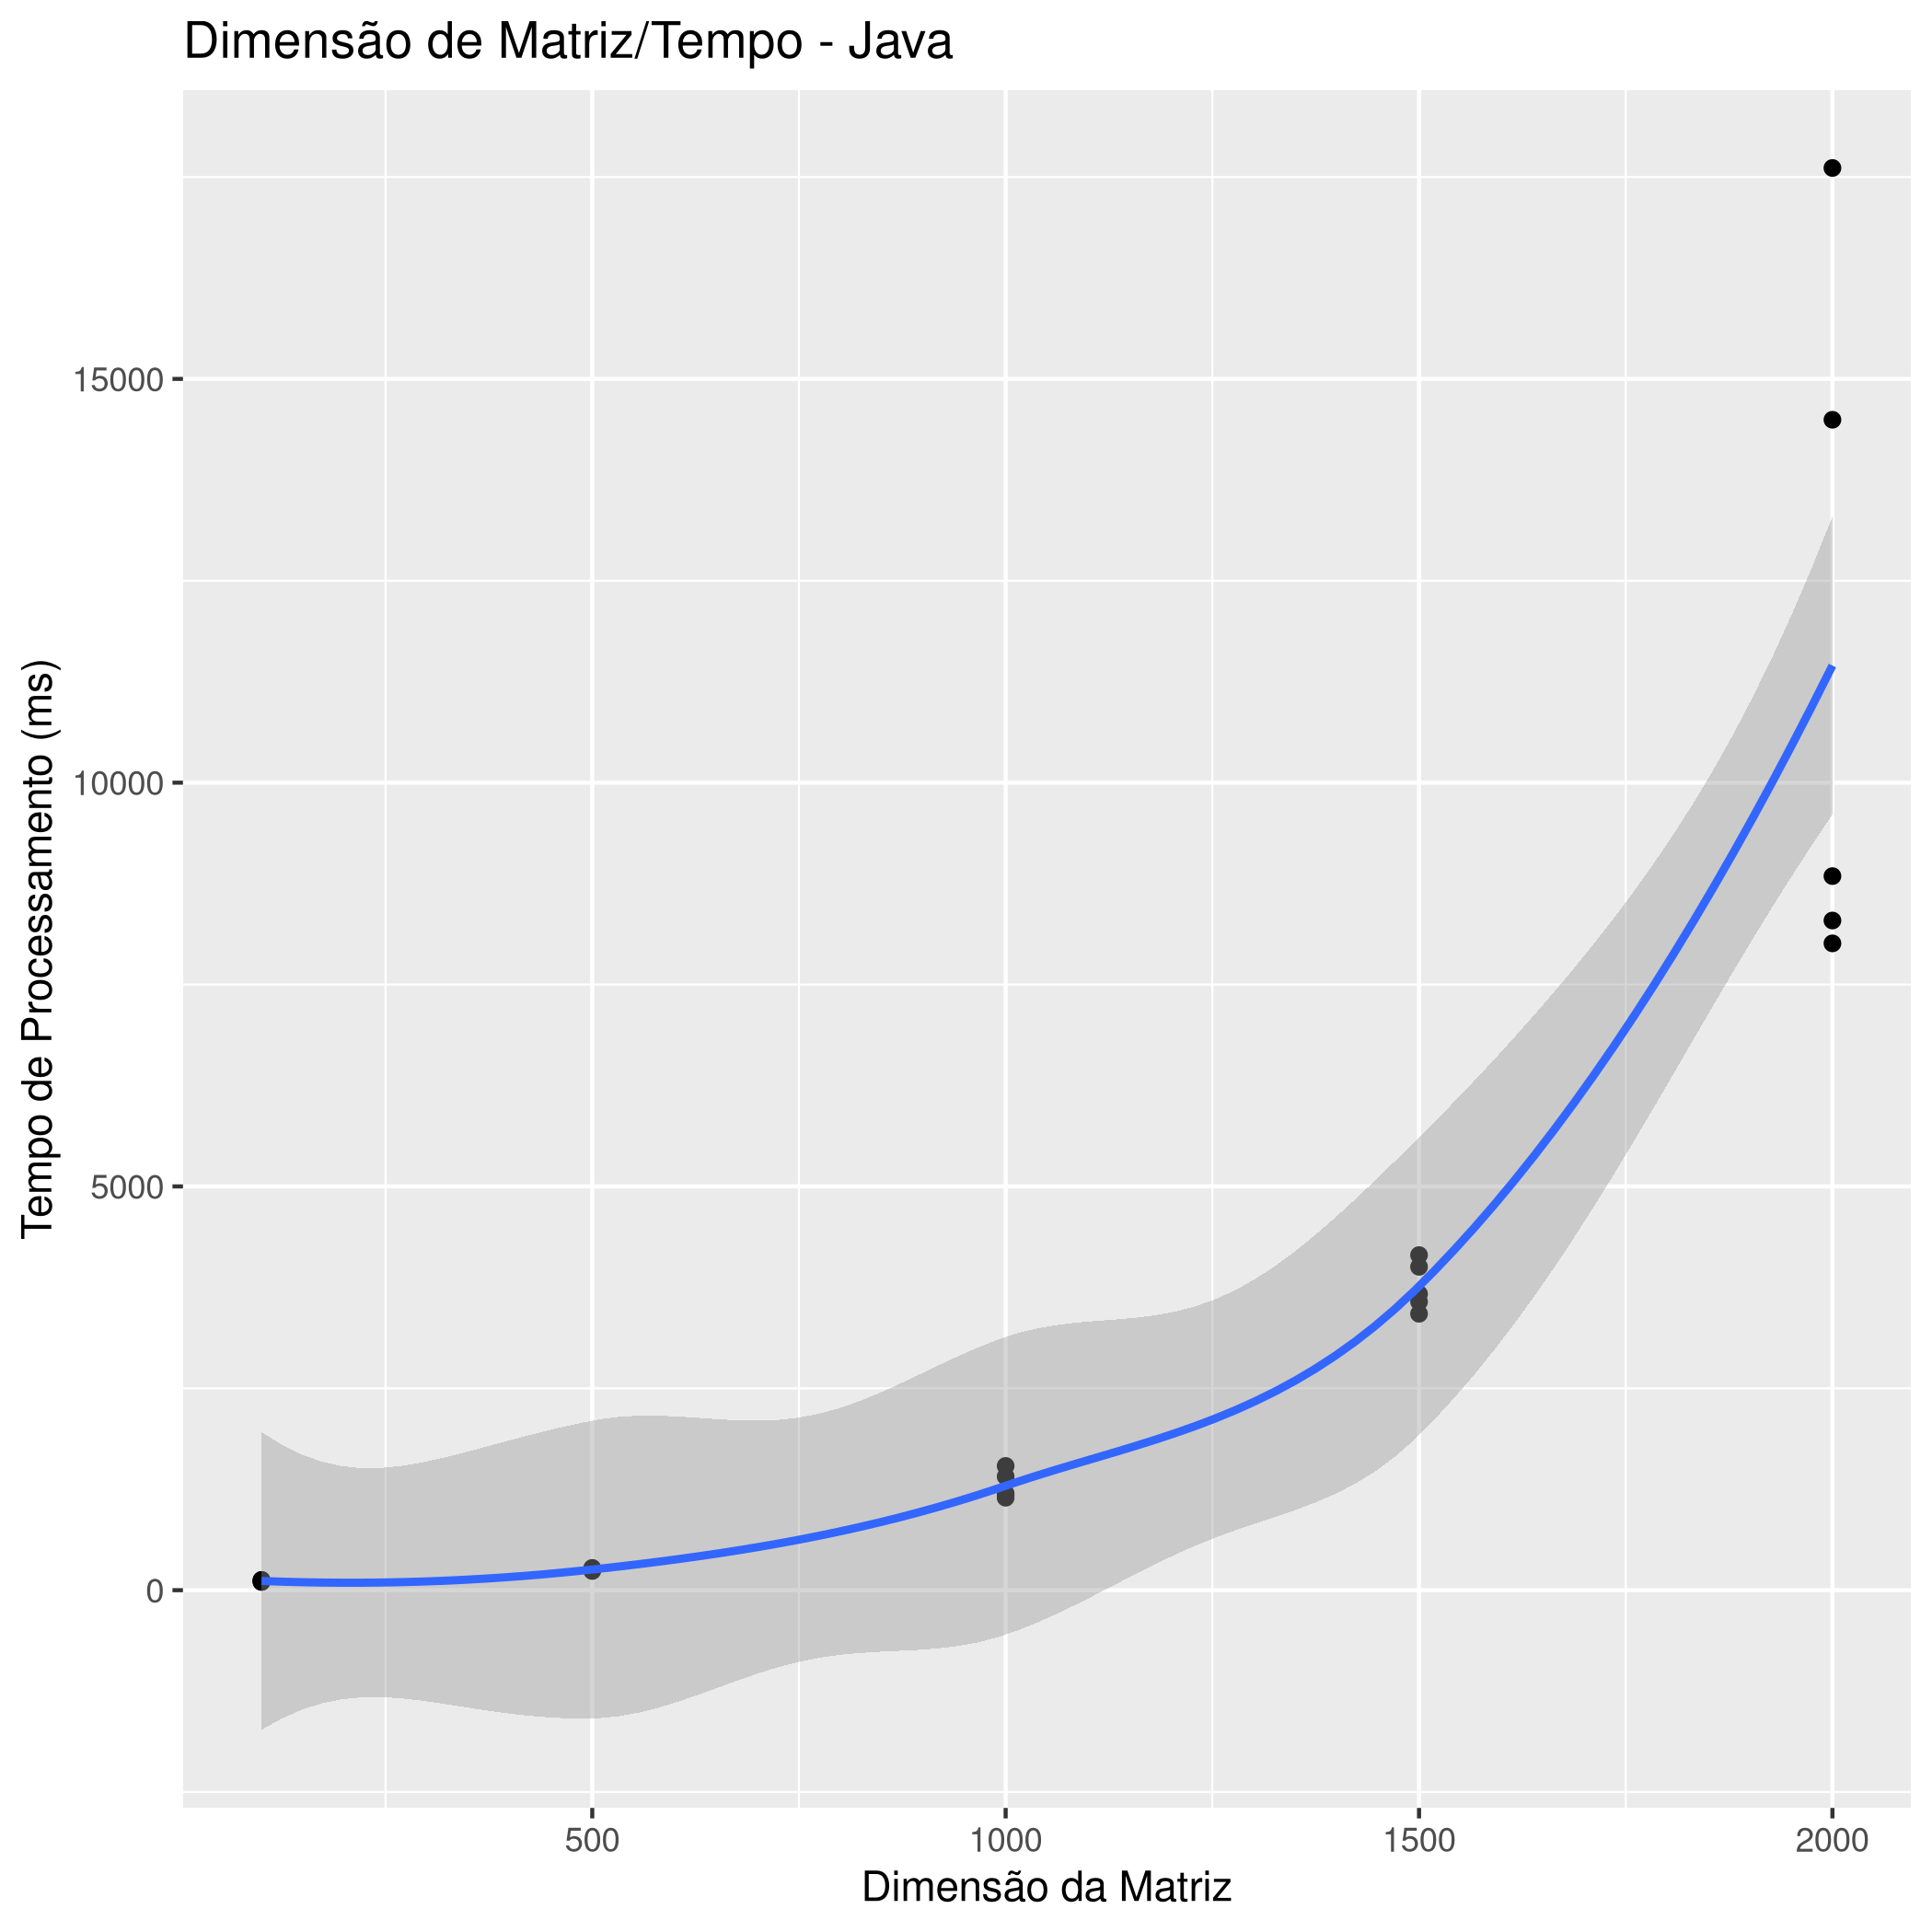
\includegraphics[width =0.3\textwidth]{plot_java.png}
    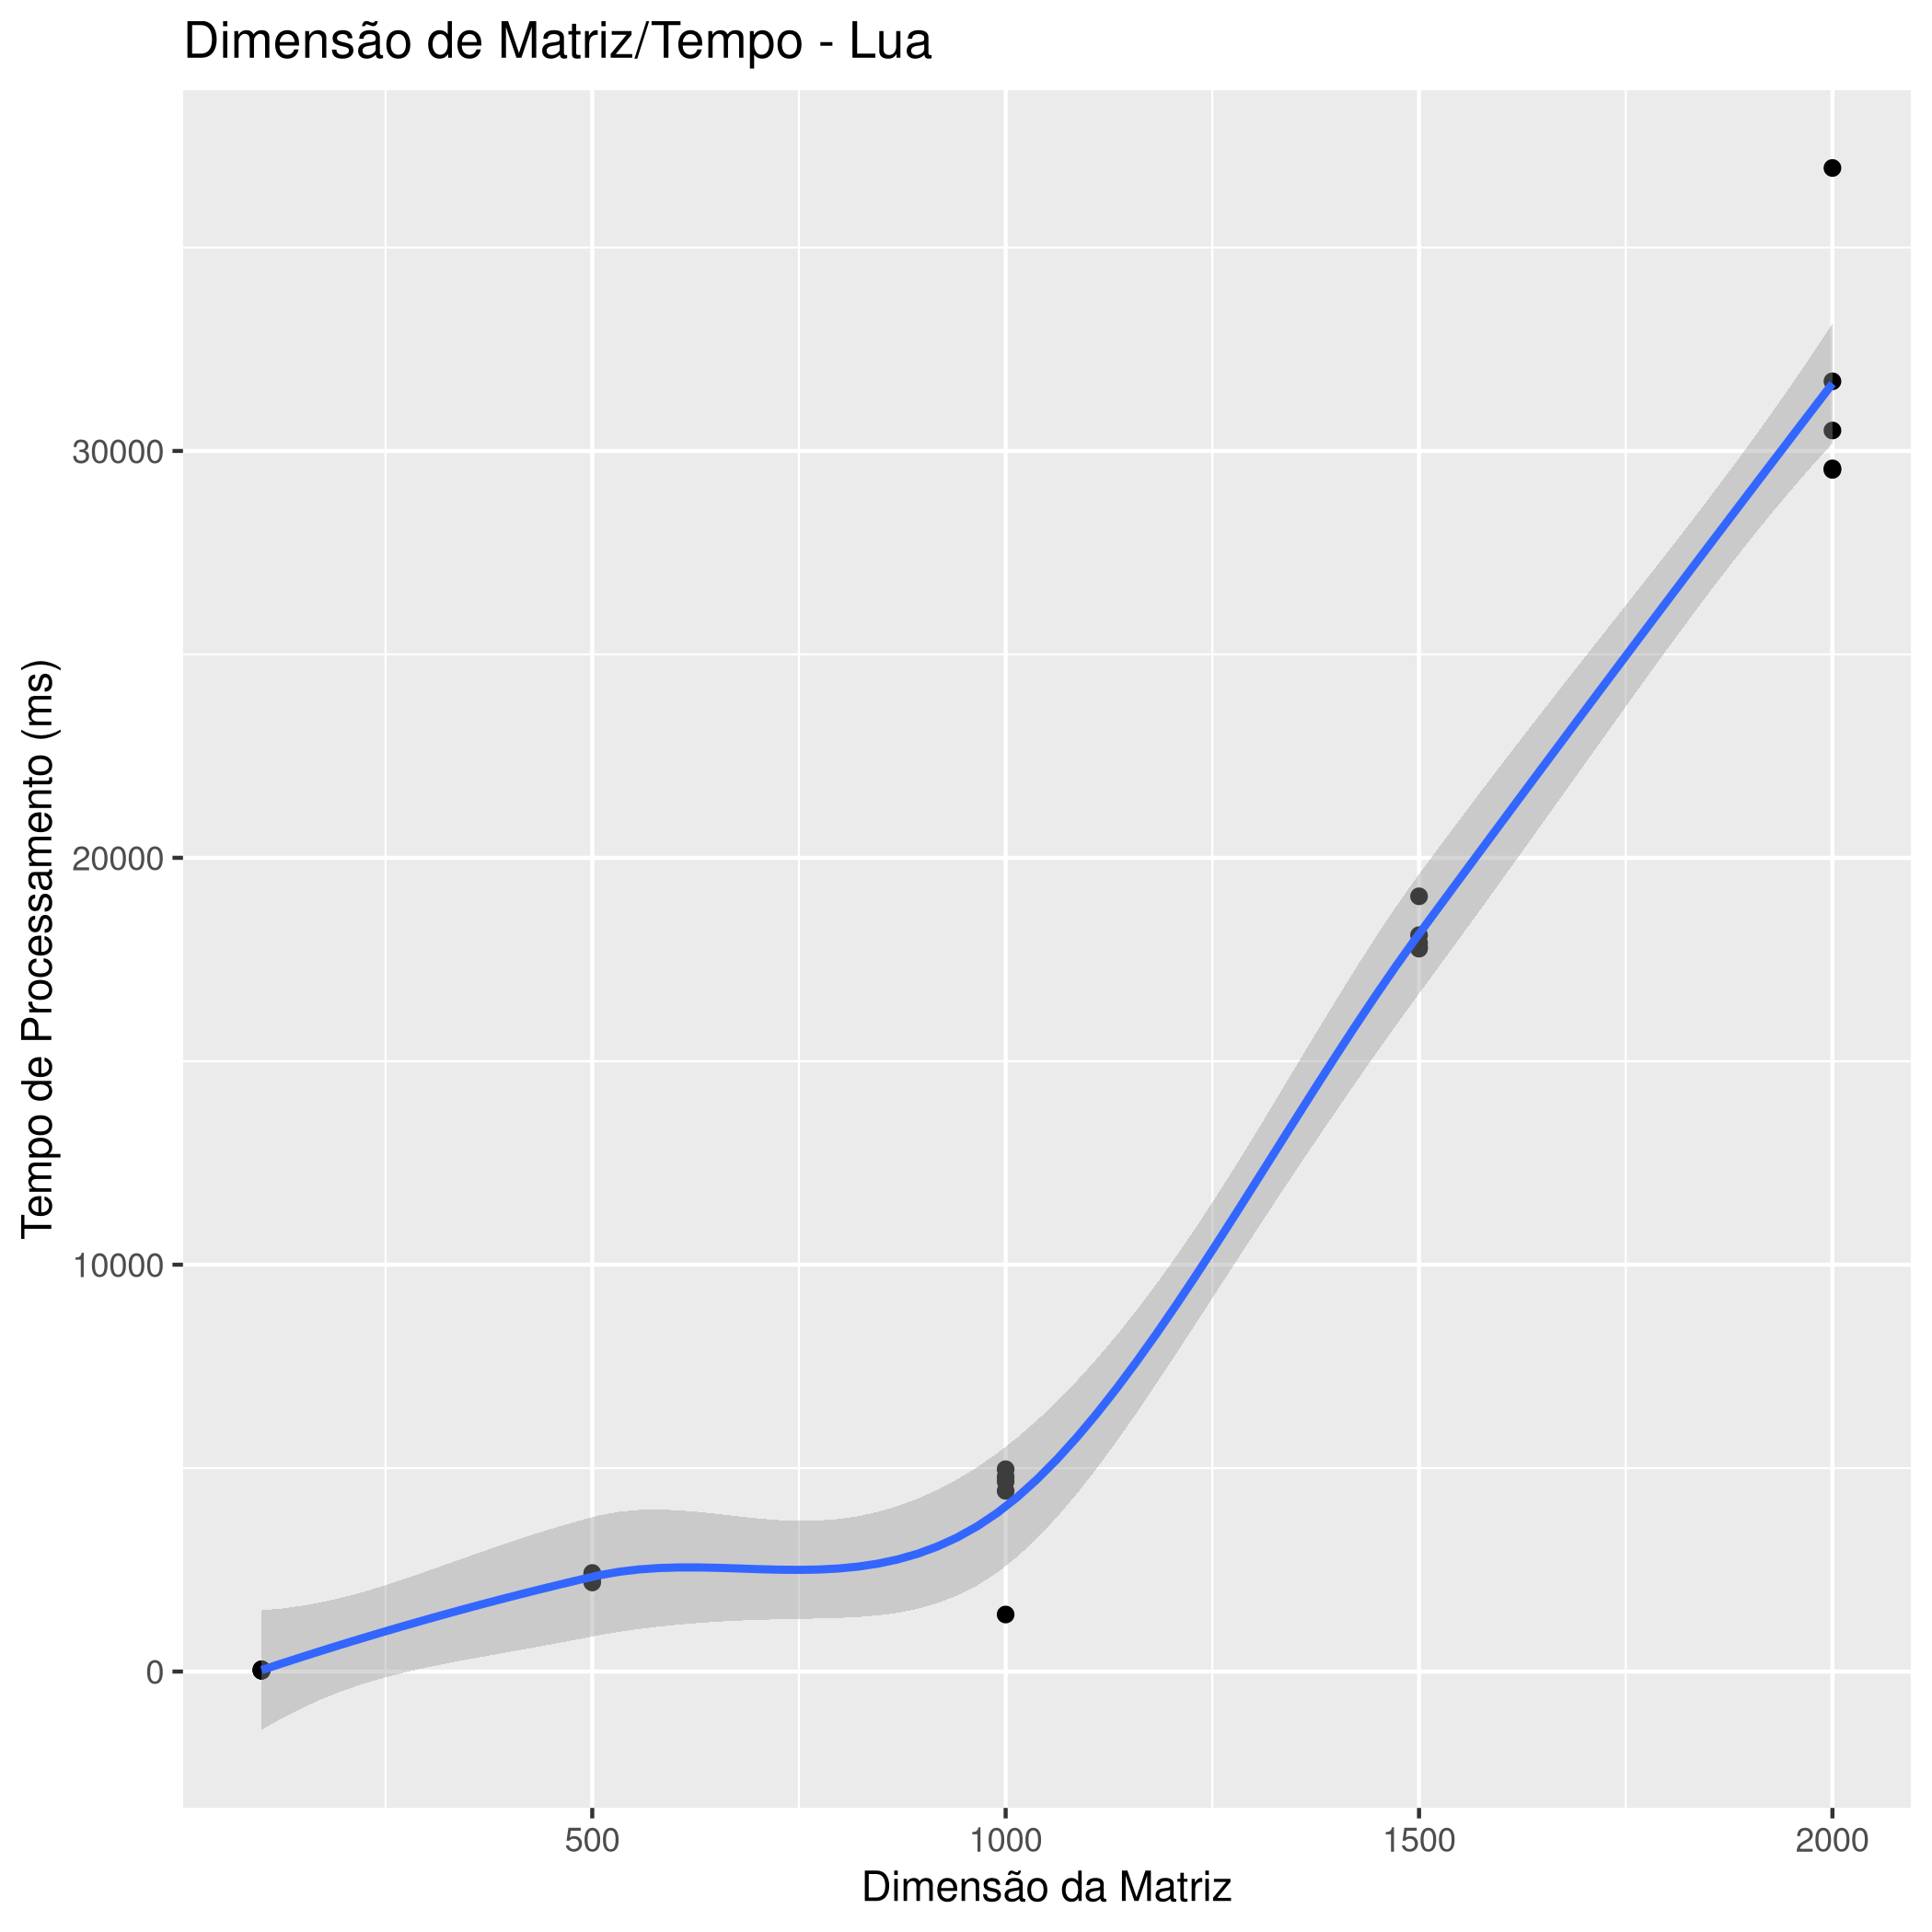
\includegraphics[width =0.3\textwidth]{plot_lua.png}
\end{figure}

\begin{figure}[!ht]
    \centering
    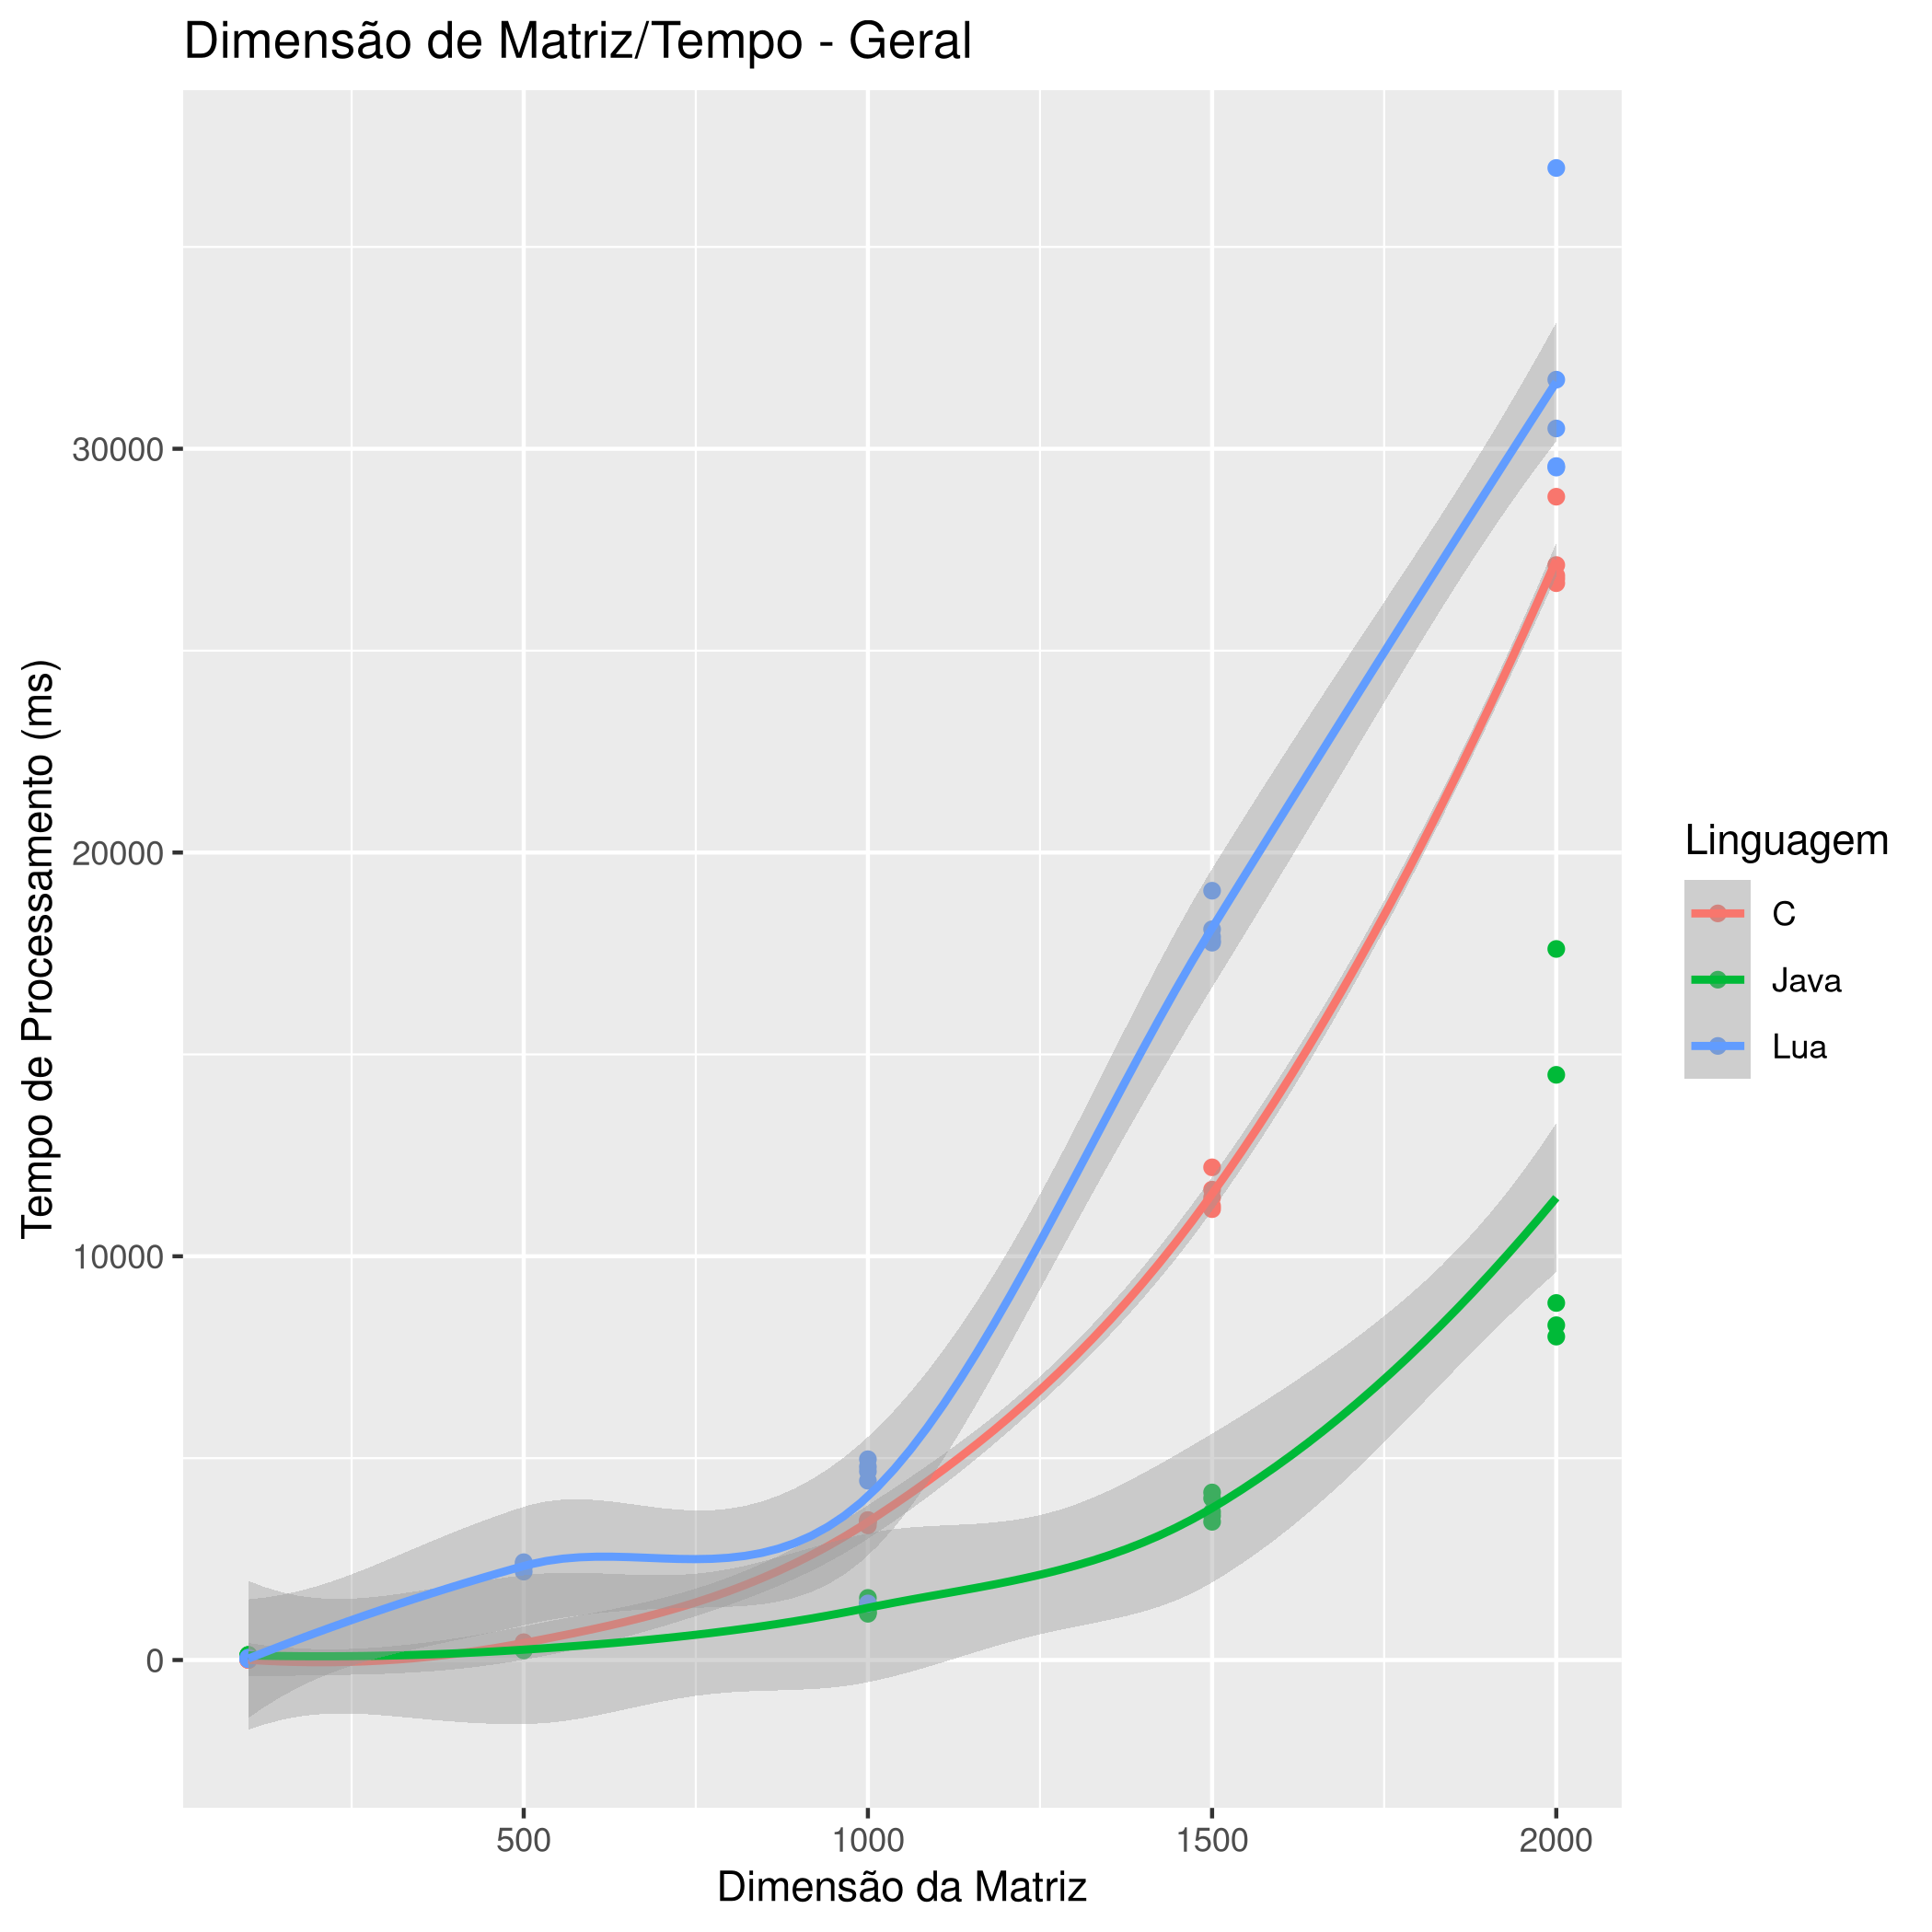
\includegraphics[width =0.49\textwidth]{plot_geral.png}
    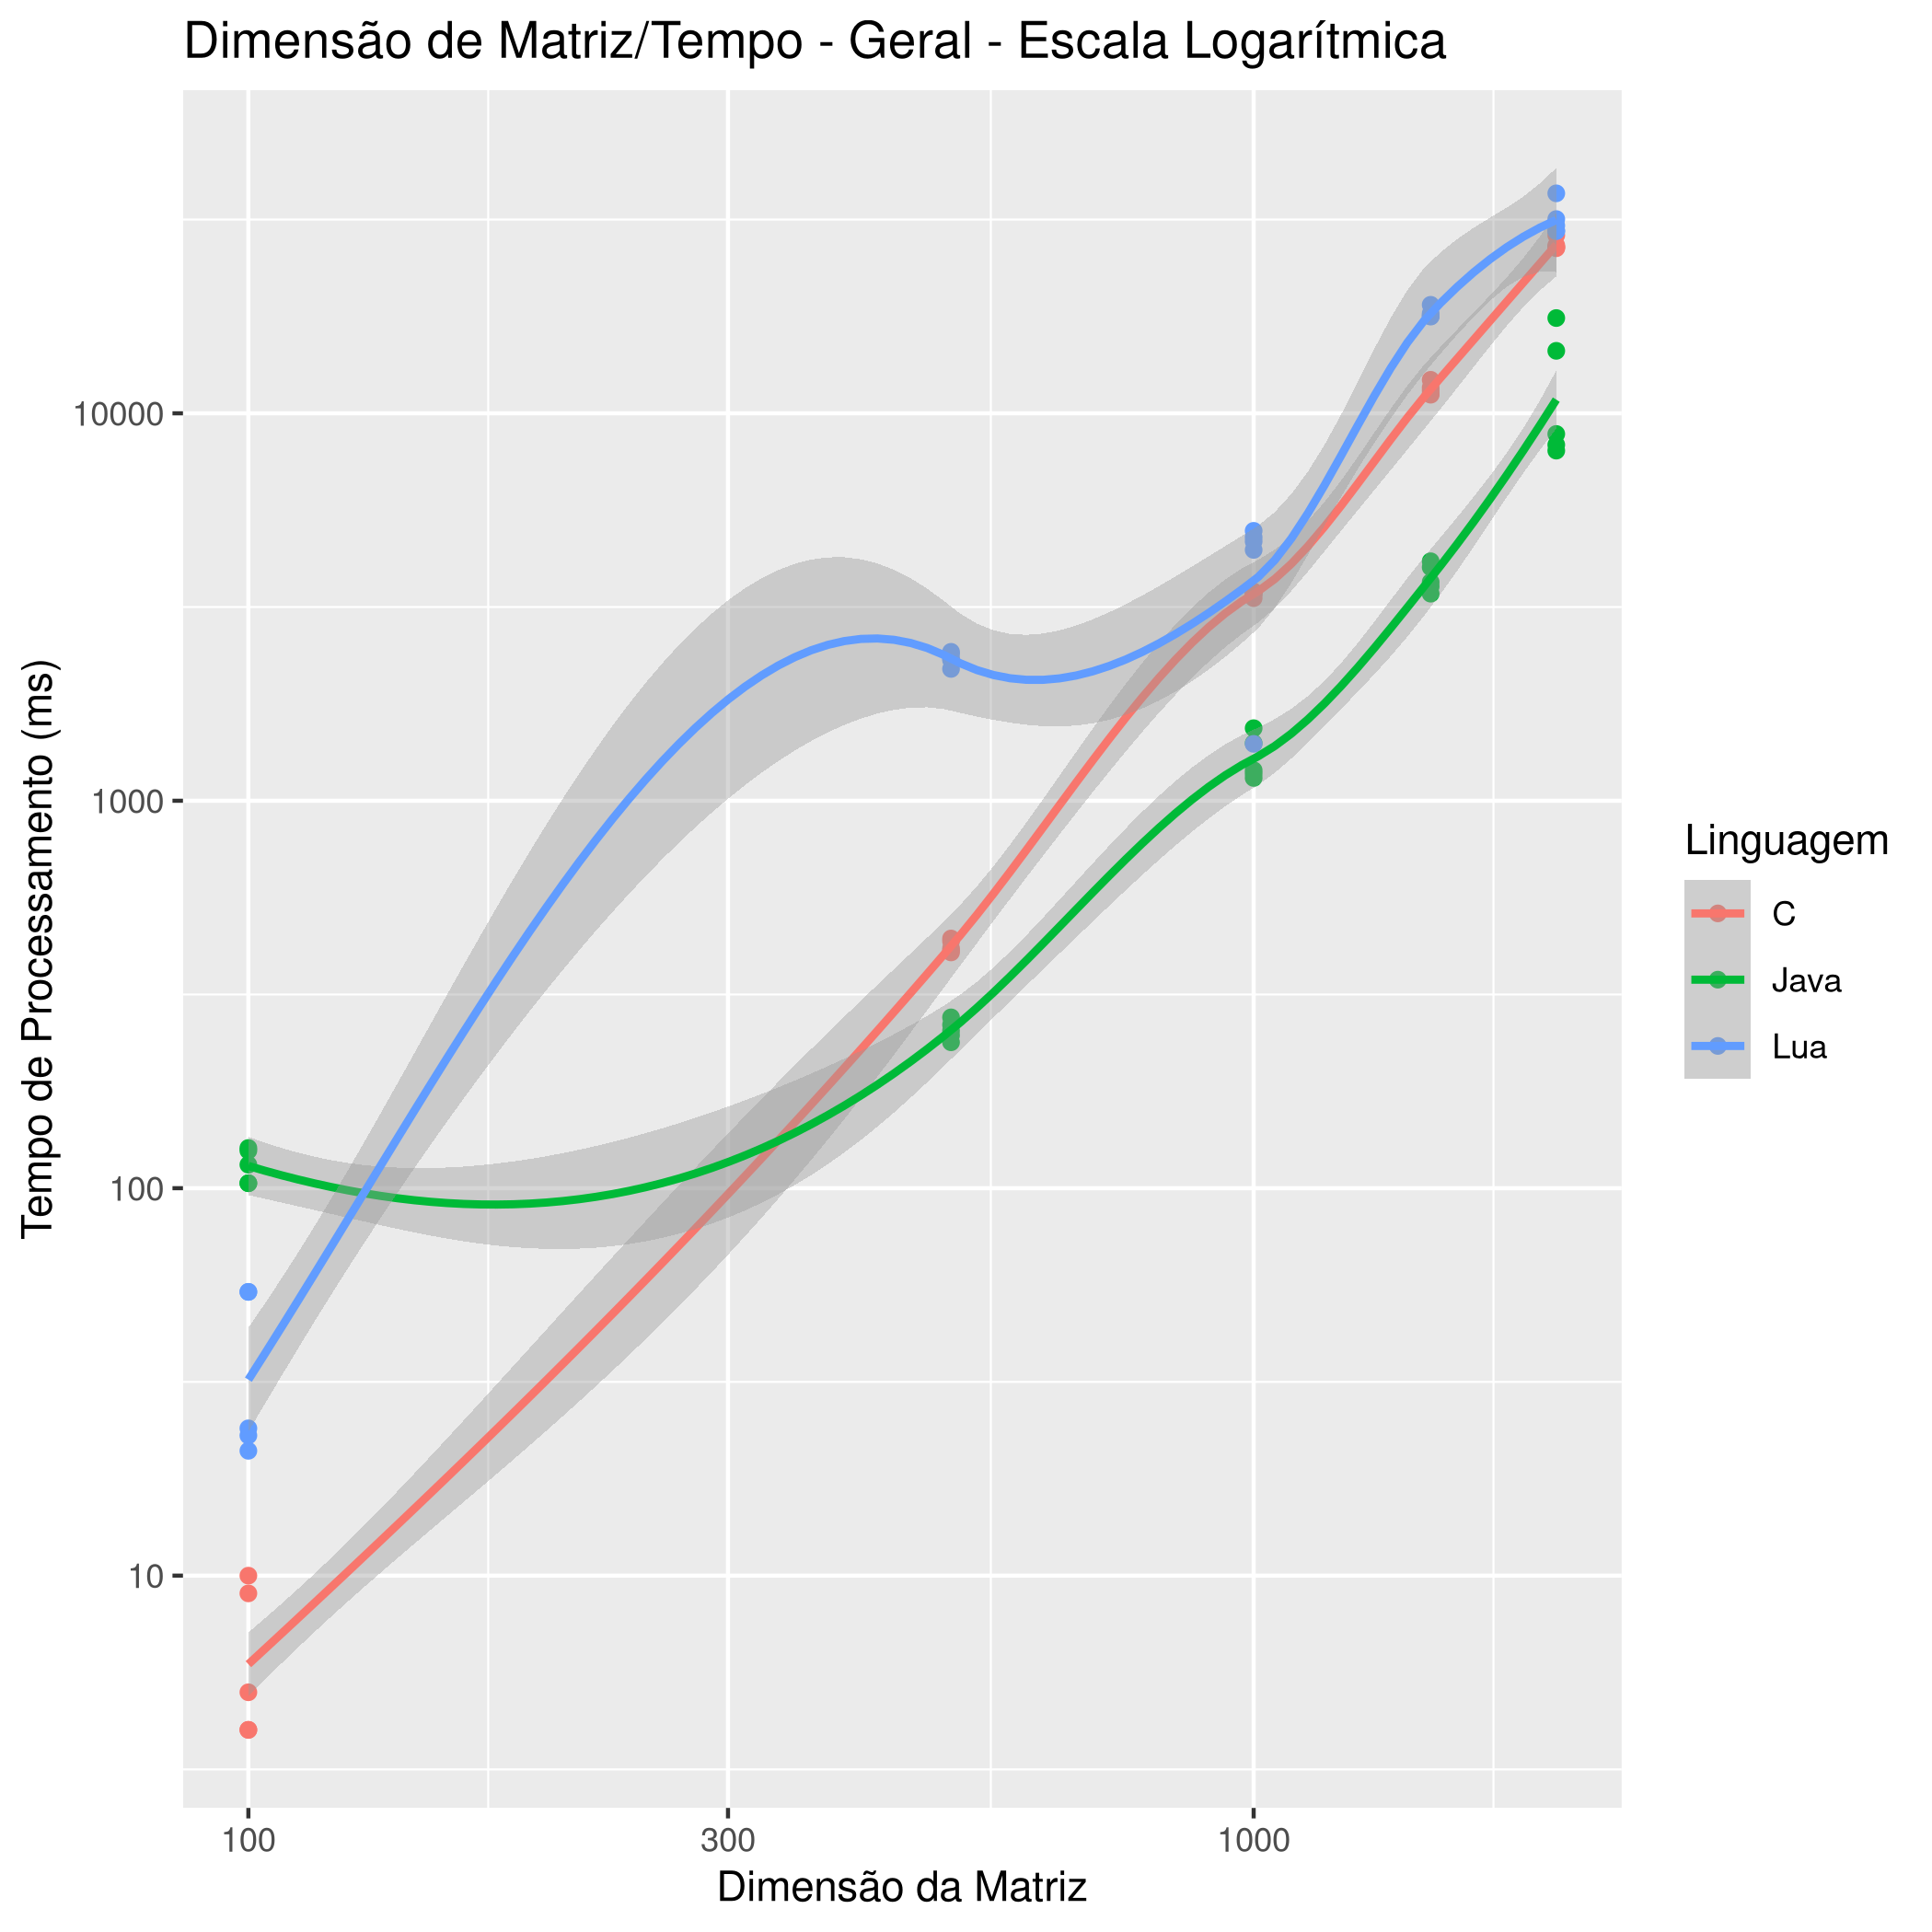
\includegraphics[width =0.49\textwidth]{plot_log.png}
\end{figure}

\newpage
\section{Conclusões Finais}
\paragraph{}

\newpage
\section{Referências Bibliográficas}
\bibliographystyle{plain}
\bibliography{references}

\end{document}
